\documentclass[14pt]{extbook}
\usepackage{multicol, enumerate, enumitem, hyperref, color, soul, setspace, parskip, fancyhdr} %General Packages
\usepackage{amssymb, amsthm, amsmath, bbm, latexsym, units, mathtools} %Math Packages
\everymath{\displaystyle} %All math in Display Style
% Packages with additional options
\usepackage[headsep=0.5cm,headheight=12pt, left=1 in,right= 1 in,top= 1 in,bottom= 1 in]{geometry}
\usepackage[usenames,dvipsnames]{xcolor}
\usepackage{dashrule}  % Package to use the command below to create lines between items
\newcommand{\litem}[1]{\item#1\hspace*{-1cm}\rule{\textwidth}{0.4pt}}
\pagestyle{fancy}
\lhead{Progress Quiz 3}
\chead{}
\rhead{Version A}
\lfoot{3148-2249}
\cfoot{}
\rfoot{Spring 2021}
\begin{document}

\begin{enumerate}
\litem{
Solve the radical equation below. Then, choose the interval(s) that the solution(s) belongs to.\[ \sqrt{12 x^2 + 64} - \sqrt{56 x} = 0 \]\begin{enumerate}[label=\Alph*.]
\item \( x_1 \in [1.37, 2.66] \text{ and } x_2 \in [1.67,3.67] \)
\item \( x_1 \in [-2.67, -2.63] \text{ and } x_2 \in [-3,1] \)
\item \( x \in [2.42,3.04] \)
\item \( x \in [1.37,2.66] \)
\item \( \text{All solutions lead to invalid or complex values in the equation.} \)

\end{enumerate} }
\litem{
What is the domain of the function below?\[ f(x) = \sqrt[4]{-6 x - 3} \]\begin{enumerate}[label=\Alph*.]
\item \( (-\infty, a], \text{ where } a \in [-0.5, 4.5] \)
\item \( [a, \infty), \text{where } a \in [-1.5, 4.5] \)
\item \( (-\infty, a], \text{where } a \in [-8, -1] \)
\item \( [a, \infty), \text{where } a \in [-2, -1] \)
\item \( (-\infty, \infty) \)

\end{enumerate} }
\litem{
Choose the graph of the equation below.\[ f(x) = \sqrt[3]{x + 8} - 7 \]\begin{enumerate}[label=\Alph*.]
\begin{multicols}{2}\item 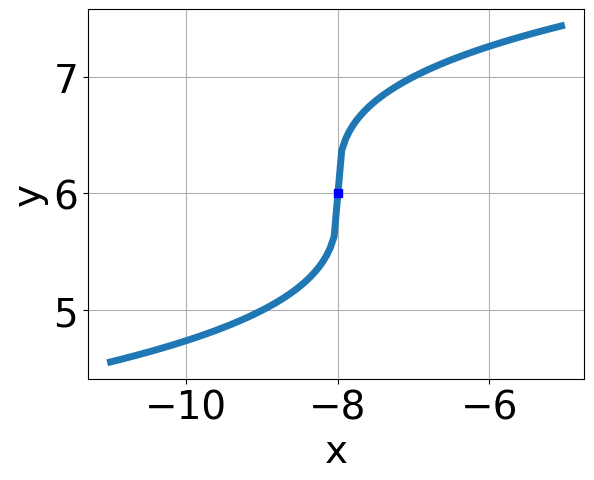
\includegraphics[width = 0.3\textwidth]{../Figures/radicalEquationToGraphAA.png}\item 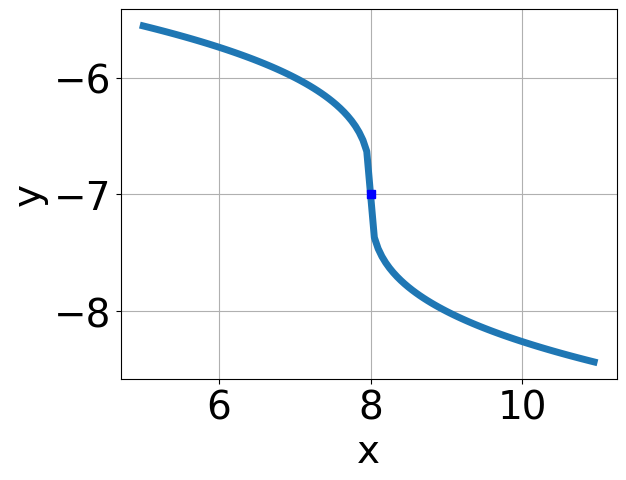
\includegraphics[width = 0.3\textwidth]{../Figures/radicalEquationToGraphBA.png}\item 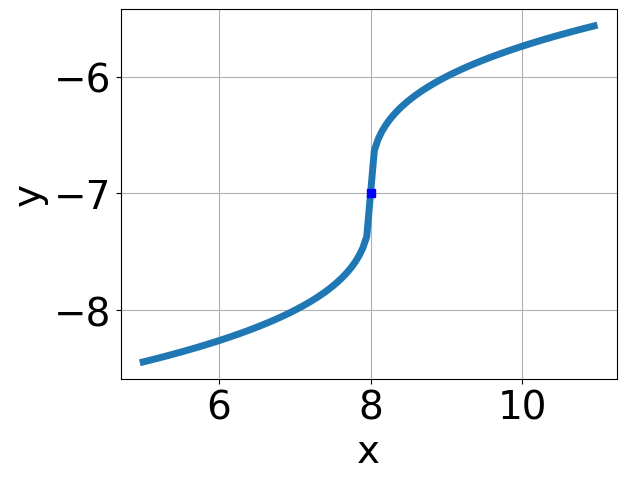
\includegraphics[width = 0.3\textwidth]{../Figures/radicalEquationToGraphCA.png}\item 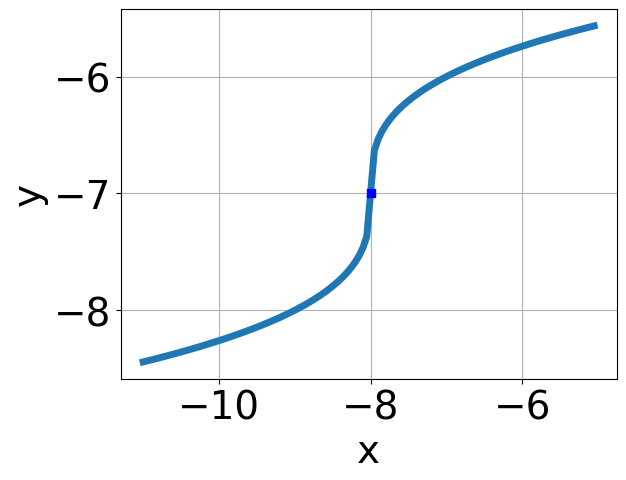
\includegraphics[width = 0.3\textwidth]{../Figures/radicalEquationToGraphDA.png}\end{multicols}\item None of the above.
\end{enumerate} }
\litem{
Choose the graph of the equation below.\[ f(x) = \sqrt[3]{x + 10} - 4 \]\begin{enumerate}[label=\Alph*.]
\begin{multicols}{2}\item 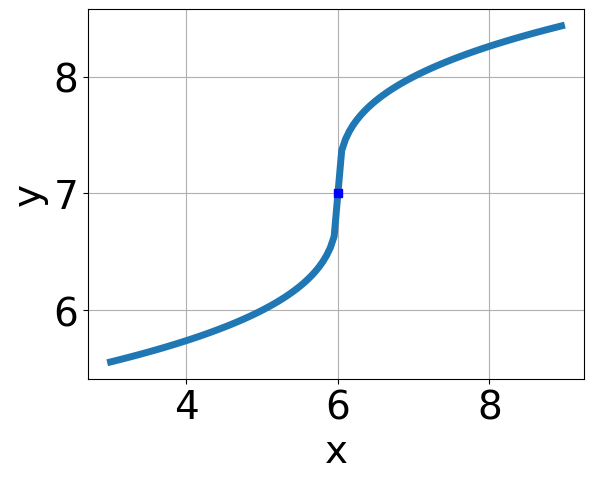
\includegraphics[width = 0.3\textwidth]{../Figures/radicalEquationToGraphCopyAA.png}\item 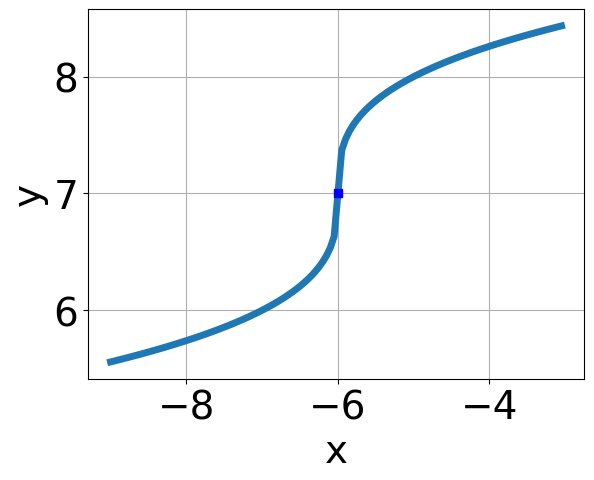
\includegraphics[width = 0.3\textwidth]{../Figures/radicalEquationToGraphCopyBA.png}\item 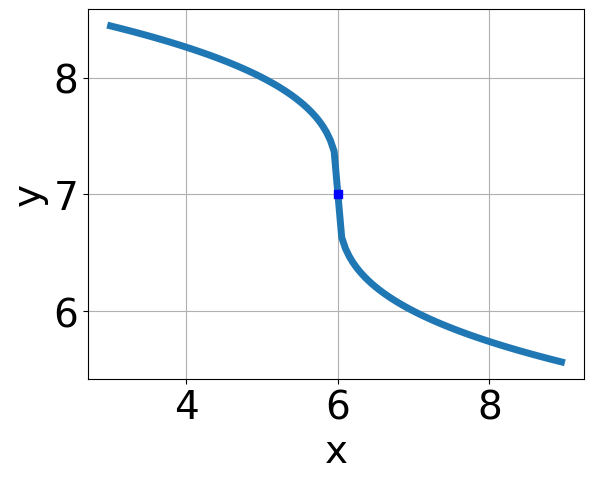
\includegraphics[width = 0.3\textwidth]{../Figures/radicalEquationToGraphCopyCA.png}\item 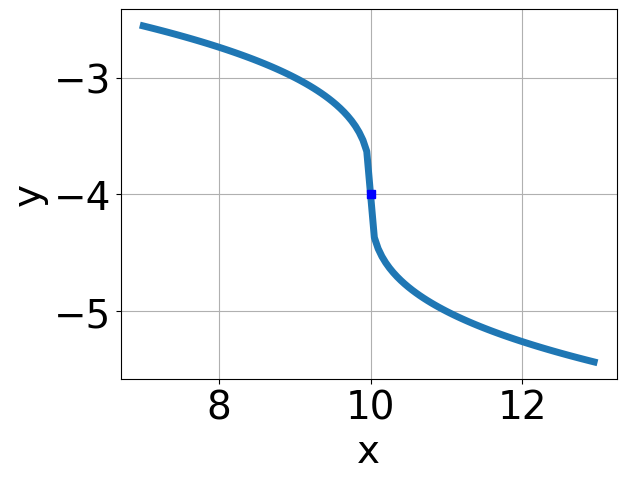
\includegraphics[width = 0.3\textwidth]{../Figures/radicalEquationToGraphCopyDA.png}\end{multicols}\item None of the above.
\end{enumerate} }
\litem{
Solve the radical equation below. Then, choose the interval(s) that the solution(s) belongs to.\[ \sqrt{35 x^2 - 16} - \sqrt{-8 x} = 0 \]\begin{enumerate}[label=\Alph*.]
\item \( x_1 \in [-3.6, 0] \text{ and } x_2 \in [0.48,0.59] \)
\item \( \text{All solutions lead to invalid or complex values in the equation.} \)
\item \( x \in [-3.6,0] \)
\item \( x \in [-0.3,1.3] \)
\item \( x_1 \in [-0.3, 1.3] \text{ and } x_2 \in [0.6,0.89] \)

\end{enumerate} }
\litem{
Solve the radical equation below. Then, choose the interval(s) that the solution(s) belongs to.\[ \sqrt{-9 x - 3} - \sqrt{4 x + 4} = 0 \]\begin{enumerate}[label=\Alph*.]
\item \( x \in [-0.22,0.19] \)
\item \( x_1 \in [-1.33, -0.64] \text{ and } x_2 \in [-1.33,1.67] \)
\item \( x \in [-0.85,-0.51] \)
\item \( \text{All solutions lead to invalid or complex values in the equation.} \)
\item \( x_1 \in [-0.85, -0.51] \text{ and } x_2 \in [-1.33,1.67] \)

\end{enumerate} }
\litem{
What is the domain of the function below?\[ f(x) = \sqrt[7]{3 x - 9} \]\begin{enumerate}[label=\Alph*.]
\item \( \text{The domain is } (-\infty, a], \text{   where } a \in [1.2, 4.8] \)
\item \( \text{The domain is } (-\infty, a], \text{   where } a \in [-0.1, 0.7] \)
\item \( (-\infty, \infty) \)
\item \( \text{The domain is } [a, \infty), \text{   where } a \in [-2.67, 2.33] \)
\item \( \text{The domain is } [a, \infty), \text{   where } a \in [1, 6] \)

\end{enumerate} }
\litem{
Choose the equation of the function graphed below.
\begin{center}
    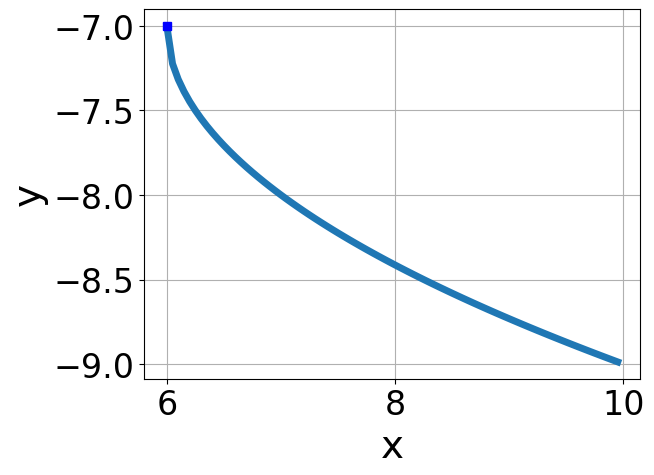
\includegraphics[width=0.5\textwidth]{../Figures/radicalGraphToEquationCopyA.png}
\end{center}
\begin{enumerate}[label=\Alph*.]
\item \( f(x) = \sqrt[3]{x + 6} - 7 \)
\item \( f(x) = - \sqrt[3]{x + 6} - 7 \)
\item \( f(x) = - \sqrt[3]{x - 6} - 7 \)
\item \( f(x) = \sqrt[3]{x - 6} - 7 \)
\item \( \text{None of the above} \)

\end{enumerate} }
\litem{
Choose the equation of the function graphed below.
\begin{center}
    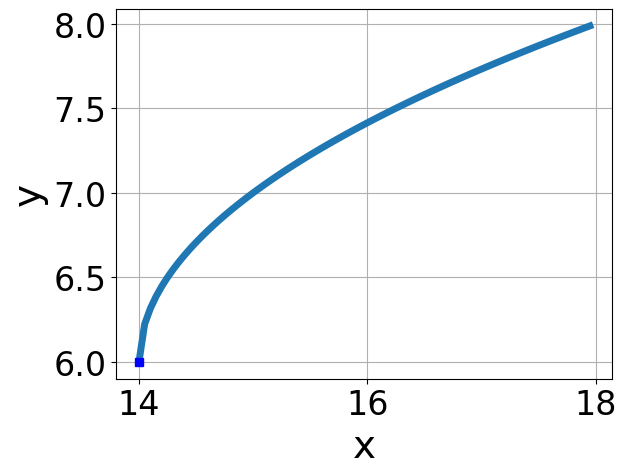
\includegraphics[width=0.5\textwidth]{../Figures/radicalGraphToEquationA.png}
\end{center}
\begin{enumerate}[label=\Alph*.]
\item \( f(x) = - \sqrt[3]{x + 14} + 6 \)
\item \( f(x) = \sqrt[3]{x + 14} + 6 \)
\item \( f(x) = \sqrt[3]{x - 14} + 6 \)
\item \( f(x) = - \sqrt[3]{x - 14} + 6 \)
\item \( \text{None of the above} \)

\end{enumerate} }
\litem{
Solve the radical equation below. Then, choose the interval(s) that the solution(s) belongs to.\[ \sqrt{-6 x + 4} - \sqrt{5 x - 5} = 0 \]\begin{enumerate}[label=\Alph*.]
\item \( x_1 \in [0.47, 0.74] \text{ and } x_2 \in [0.95,1.22] \)
\item \( x \in [-0.41,0.22] \)
\item \( x_1 \in [0.47, 0.74] \text{ and } x_2 \in [0.64,0.89] \)
\item \( \text{All solutions lead to invalid or complex values in the equation.} \)
\item \( x \in [0.8,1.15] \)

\end{enumerate} }
\end{enumerate}

\end{document}